\documentclass[a4paper,12pt]{article}

%%% Alapdokumentum beállítások %%%
\usepackage[hungarian]{babel}
\usepackage[T1]{fontenc}
\usepackage[utf8]{inputenc}
\usepackage{geometry}
\geometry{a4paper, margin=1.2in}

%%% Szövegformázás és elrendezés %%%
\usepackage{microtype}
\usepackage{parskip}
\usepackage{enumitem}
\usepackage{multicol}
\setlength{\emergencystretch}{3em}

%%% Matematikai csomagok %%%
\usepackage{amsmath, amssymb, amsfonts, amsthm}

%%% Színek és dobozok %%%
\usepackage{xcolor}
\definecolor{mainblue}{rgb}{0.1, 0.35, 0.65}
\definecolor{maingreen}{rgb}{0.12, 0.55, 0.25}
\definecolor{mainorange}{rgb}{0.85, 0.42, 0.05}
\definecolor{bvred}{rgb}{0.8, 0.0, 0.0}

\usepackage{tcolorbox}
\tcbuselibrary{theorems,skins,breakable}
\usepackage{booktabs}
\usepackage{float}
\usepackage{caption}

%%% TikZ ábrák %%%
\usepackage{tikz}
\usetikzlibrary{calc, arrows.meta, positioning}

\tikzset{
    % Pötty stílus csúcsokhoz a felhasználói szabálynak megfelelően (betűk és zavaró feliratok nélkül)
    dot/.style={circle, fill=black, inner sep=2.5pt},
    highlightdot/.style={circle, fill=bvred, inner sep=3.2pt},
    % Betűs csúcs kizárólag oda, ahol a szöveg kifejezetten hivatkozik a csúcs betűjelére
    labeledvertex/.style={circle, draw=black, fill=white, thick, minimum size=18pt, inner sep=0pt, font=\small},
    labeledoddvertex/.style={circle, draw=bvred, fill=red!15, very thick, minimum size=18pt, inner sep=0pt, font=\small\bfseries},
    edge/.style={thick, draw=black!75},
    highlightedge/.style={very thick, draw=bvred},
    patharrow/.style={-latex, very thick, draw=mainblue}
}

%%% Speciális Microlearning dobozok %%%
\newtcolorbox{definiciodoboz}[1][]{colback=blue!4!white,colframe=mainblue,fonttitle=\bfseries,title=Definíció: #1}
\newtcolorbox{teteldoboz}[1][]{colback=green!6!white,colframe=maingreen,fonttitle=\bfseries,title=Tétel: #1}
\newtcolorbox{feladatdoboz}[1][]{colback=orange!5!white,colframe=mainorange,fonttitle=\bfseries,title=Megértést ellenőrző feladat: #1}
\newtcolorbox{megoldasdoboz}[1][]{colback=gray!5!white,colframe=gray!60!black,fonttitle=\bfseries,title=Megoldás és magyarázat: #1}
\newtcolorbox{tippdoboz}[1][]{colback=yellow!8!white,colframe=orange!80!black,fonttitle=\bfseries,title=Fontos megjegyzés: #1}

\usepackage{hyperref}

\title{Gráfok -- Interaktív Mikrotananyag}
\author{AI LaTeX Studio}
\date{\today}

\begin{document}

\maketitle

\begin{center}
    \textit{Módszertan: Aprózott elméleti egységek (Microlearning) $\longrightarrow$ Azonnali ellenőrző feladatok (A/B/C/D, Igaz/Hamis, Számolás, Többlépcsős vezetés).}
\end{center}

\vspace{0.5cm}

% ==============================================================================
% 1. EGYSÉG: GRÁF FOGALMA
% ==============================================================================
\section{1. Mikro-egység: Mi az a gráf?}

A gráfelméletben objektumokat és a köztük fennálló kapcsolatokat vizsgálunk.

\begin{definiciodoboz}[Gráf fogalma]
Egy $G = (V, E)$ \textbf{gráf} nem más, mint csúcsok egy nem üres $V$ halmaza (\textit{vertex}), és a csúcspárokat összekötő $E$ élek halmaza (\textit{edge}).
\end{definiciodoboz}

Az alábbi ábrán egy 4 csúcsból és 4 élből álló hálózat látható:

\begin{figure}[H]
    \centering
    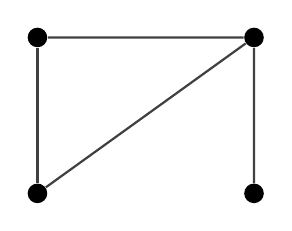
\begin{tikzpicture}[scale=1.1]
        \node[dot] (1) at (0, 1.8) {};
        \node[dot] (2) at (2.5, 1.8) {};
        \node[dot] (3) at (0, 0) {};
        \node[dot] (4) at (2.5, 0) {};

        \draw[edge] (1) -- (2);
        \draw[edge] (1) -- (3);
        \draw[edge] (2) -- (3);
        \draw[edge] (2) -- (4);
    \end{tikzpicture}
    \caption{Egy egyszerű hálózat pontként ábrázolt csúcsokkal és élekkel.}
\end{figure}

\begin{feladatdoboz}[1. Kérdés: Feleletválasztós (A/B/C/D)]
Egy ország vasúti hálózatának gráfmodelljében minek felelnek meg a vasútállomások és a köztük lévő közvetlen vasúti sínek?
\begin{enumerate}[label=(\Alph*)]
    \item Az állomások az élek, a sínek a csúcsok.
    \item Az állomások a csúcsok, a sínek az élek.
    \item Mindkettő élnek minősül.
    \item Egyik sem, vasúti hálózatot nem lehet gráffal ábrázolni.
\end{enumerate}
\end{feladatdoboz}

\begin{megoldasdoboz}[Megoldás az 1. feladathoz]
\textbf{Helyes válasz: (B)} \\
Az objektumok (a városok/állomások) a gráf csúcsai ($V$), míg a köztük futó fizikai kapcsolatok (a vasúti sínek) az élek ($E$).
\end{megoldasdoboz}

\vspace{0.4cm}
% ==============================================================================
% 2. EGYSÉG: FOKSZÁM
% ==============================================================================
\section{2. Mikro-egység: A csúcs fokszáma}

\begin{definiciodoboz}[Fokszám]
Egy csúcs \textbf{fokszáma} az adott csúcsba befutó (abból kiinduló) élek száma. \\
Jelölése: $d(v)$ (az angol \textit{degree} szóból).
\end{definiciodoboz}

Képzeld el úgy, mintha egy társasági összejövetelen megkérdeznénk valakit: \textit{„Hány emberrel fogtál kezet?”}

\begin{figure}[H]
    \centering
    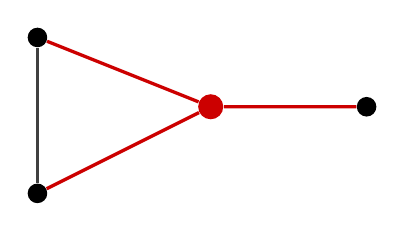
\begin{tikzpicture}[scale=1.1]
        \node[dot] (a) at (0, 1.8) {};
        \node[highlightdot] (center) at (2, 1) {};
        \node[dot] (c) at (0, 0) {};
        \node[dot] (d) at (3.8, 1) {};

        \draw[highlightedge] (center) -- (a);
        \draw[highlightedge] (center) -- (c);
        \draw[highlightedge] (center) -- (d);
        \draw[edge] (a) -- (c);
    \end{tikzpicture}
    \caption{A piros ponttal jelölt csúcsból pontosan 3 él fut ki, míg a többiekből kevesebb.}
\end{figure}

\begin{feladatdoboz}[2. Kérdés: Konkrét számérték megadása]
Nézd meg a fenti ábrát! Határozd meg a pirossal kiemelt csúcs fokszámát, valamint a jobb szélső csúcs fokszámát!
\end{feladatdoboz}

\begin{megoldasdoboz}[Megoldás a 2. feladathoz]
\textbf{Eredmény:}
\begin{itemize}
    \item A kiemelt középső csúcsból 3 él indul ki, így fokszáma: $\mathbf{d = 3}$.
    \item A jobb szélső csúcsba mindössze egyetlen vonal fut be, így annak fokszáma: $\mathbf{d = 1}$.
\end{itemize}
\end{megoldasdoboz}

\vspace{0.4cm}
% ==============================================================================
% 3. EGYSÉG: EGYSZERŰ GRÁFOK
% ==============================================================================
\section{3. Mikro-egység: Egyszerű gráf vs. Hurokél és Többszörös él}

\begin{definiciodoboz}[Egyszerű gráf]
Egy gráfot \textbf{egyszerűnek} nevezünk, ha nem tartalmaz:
\begin{itemize}
    \item \textbf{hurokélt} (olyan él, amely egy csúcsot önmagával köt össze),
    \item és nem tartalmaz \textbf{többszörös (párhuzamos) éleket} (két csúcs között legfeljebb egyetlen él futhat).
\end{itemize}
\end{definiciodoboz}

Középiskolában szinte kivétel nélkül egyszerű gráfokkal foglalkozunk.

\begin{figure}[H]
    \centering
    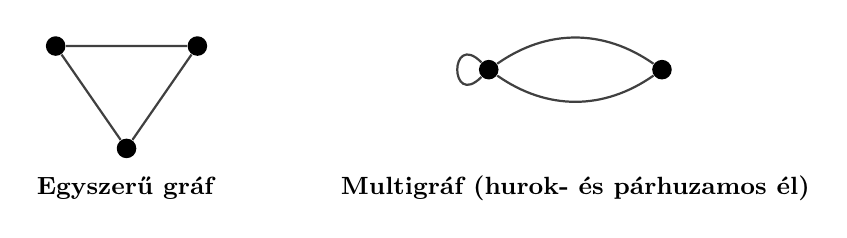
\begin{tikzpicture}[scale=1.0]
        % Egyszerű
        \begin{scope}[xshift=0cm]
            \node[dot] (p1) at (0, 1.3) {};
            \node[dot] (p2) at (1.8, 1.3) {};
            \node[dot] (p3) at (0.9, 0) {};
            \draw[edge] (p1) -- (p2) -- (p3) -- (p1);
            \node at (0.9, -0.5) {\small \textbf{Egyszerű gráf}};
        \end{scope}

        % Nem egyszerű
        \begin{scope}[xshift=5.5cm]
            \node[dot] (u) at (0, 1) {};
            \node[dot] (v) at (2.2, 1) {};
            \draw[edge] (u) to[bend left=35] (v);
            \draw[edge] (u) to[bend right=35] (v);
            \draw[edge] (u) to[out=135, in=225, looseness=8] (u);
            \node at (1.1, -0.5) {\small \textbf{Multigráf (hurok- és párhuzamos él)}};
        \end{scope}
    \end{tikzpicture}
    \caption{Egyszerű gráf és nem egyszerű gráf összevetése.}
\end{figure}

\begin{feladatdoboz}[3. Kérdés: Igaz / Hamis állítások]
Döntsd el az alábbi állításokról, hogy Igazak (I) vagy Hamisak (H)!
\begin{enumerate}[label=\alph*)]
    \item Egy egyszerű gráfban előfordulhat, hogy két ismerős között két független ismeretségi él fut.
    \item Egy egyszerű gráfban senki sem foghat kezet önmagával (nincs hurokél).
    \item Egy $n$ csúcsú egyszerű gráfban egyetlen csúcs fokszáma sem haladhatja meg az $n-1$-et.
\end{enumerate}
\end{feladatdoboz}

\begin{megoldasdoboz}[Megoldás a 3. feladathoz]
\begin{itemize}
    \item \textbf{a) Hamis:} Egyszerű gráfban két csúcs között legfeljebb egyetlen él lehet (nincsenek többszörös élek).
    \item \textbf{b) Igaz:} A hurokél kizárt az egyszerű gráf definíciója szerint.
    \item \textbf{c) Igaz:} Mivel nincsenek hurkok és párhuzamos élek, egy csúcs legfeljebb a nála lévő összes többi $n-1$ csúccsal lehet összekötve.
\end{itemize}
\end{megoldasdoboz}

\vspace{0.4cm}
% ==============================================================================
% 4. EGYSÉG: ÚT ÉS KÖR
% ==============================================================================
\section{4. Mikro-egység: Séta a gráfban: Út és Kör}

\begin{definiciodoboz}[Út és Kör]
\begin{itemize}
    \item \textbf{Út:} Egymáshoz csatlakozó élek olyan sorozata, ahol \textbf{egyetlen csúcsot sem érintünk kétszer}.
    \item \textbf{Kör:} Olyan zárt út, amely ugyanabba a csúcsba érkezik vissza, ahonnan elindult, és útközben semmilyen más csúcsot nem érint kétszer.
\end{itemize}
\end{definiciodoboz}

\begin{figure}[H]
    \centering
    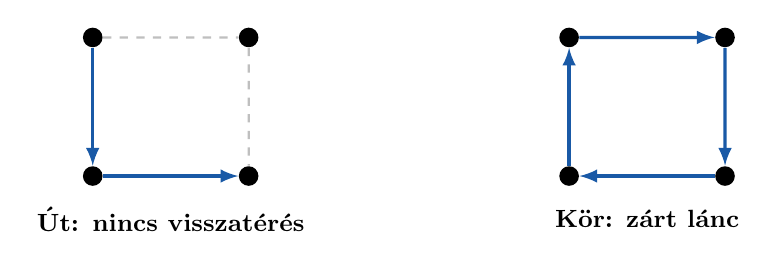
\begin{tikzpicture}[scale=1.1]
        % Út
        \begin{scope}[xshift=0cm]
            \node[dot] (a1) at (0, 1.6) {};
            \node[dot] (a2) at (1.8, 1.6) {};
            \node[dot] (a3) at (0, 0) {};
            \node[dot] (a4) at (1.8, 0) {};
            \draw[edge, dashed, black!25] (a1) -- (a2) -- (a4);
            \draw[patharrow] (a1) -- (a3);
            \draw[patharrow] (a3) -- (a4);
            \node at (0.9, -0.5) {\small \textbf{Út: nincs visszatérés}};
        \end{scope}

        % Kör
        \begin{scope}[xshift=5.5cm]
            \node[dot] (k1) at (0, 1.6) {};
            \node[dot] (k2) at (1.8, 1.6) {};
            \node[dot] (k3) at (0, 0) {};
            \node[dot] (k4) at (1.8, 0) {};
            \draw[patharrow] (k1) -- (k2);
            \draw[patharrow] (k2) -- (k4);
            \draw[patharrow] (k4) -- (k3);
            \draw[patharrow] (k3) -- (k1);
            \node at (0.9, -0.5) {\small \textbf{Kör: zárt lánc}};
        \end{scope}
    \end{tikzpicture}
    \caption{Nyílt útvonal (út) és önmagába záródó kör összehasonlítása.}
\end{figure}

\begin{feladatdoboz}[4. Kérdés: Feleletválasztós (A/B/C/D)]
Egy 5 csúcsból álló körben ($C_5$) mennyi a csúcsok száma és az élek száma?
\begin{enumerate}[label=(\Alph*)]
    \item 5 csúcs és 4 él
    \item 5 csúcs és 5 él
    \item 5 csúcs és 10 él
    \item 4 csúcs és 5 él
\end{enumerate}
\end{feladatdoboz}

\begin{megoldasdoboz}[Megoldás a 4. feladathoz]
\textbf{Helyes válasz: (B)} \\
Egy körgráfban mindig pontosan megegyezik a csúcsok és élek száma: az 5 csúcsot egymás után összekötve, majd az utolsót az elsővel zárva pontosan 5 élt kapunk.
\end{megoldasdoboz}

\vspace{0.4cm}
% ==============================================================================
% 5. EGYSÉG: ÖSSZEFÜGGŐ GRÁFOK ÉS KOMPONENSEK
% ==============================================================================
\section{5. Mikro-egység: Összefüggő gráfok}

\begin{definiciodoboz}[Összefüggőség]
Egy gráfot \textbf{összefüggőnek} nevezünk, ha bármely két csúcsa között vezet út (a gráf „egy darabban van”). \\
Ha a gráf különálló részekre esik szét, akkor nem összefüggő, és a részeit \textbf{komponenseknek} hívjuk.
\end{definiciodoboz}

\begin{feladatdoboz}[5. Kérdés: Igaz/Hamis és Rövid válasz]
\textbf{A) Igaz vagy Hamis?} Egy összefüggő gráfban mindig el lehet jutni bármelyik csúcsból bármelyik másikba élek mentén haladva. \\
\textbf{B) Rövid válasz:} Ha egy 6 csúcsú gráf két különálló 3-as körből áll, hány komponense van a gráfnak?
\end{feladatdoboz}

\begin{megoldasdoboz}[Megoldás az 5. feladathoz]
\textbf{A) Igaz:} Ez maga az összefüggőség definíciója. \\
\textbf{B) 2 komponense van}, mivel a két kör között nem fut semmilyen él, így a gráf két független darabból áll.
\end{megoldasdoboz}

\vspace{0.4cm}
% ==============================================================================
% 6. EGYSÉG: IZOMORFIA
% ==============================================================================
\section{6. Mikro-egység: Gráfok izomorfiája}

\begin{definiciodoboz}[Izomorf gráfok]
Két gráf \textbf{izomorf}, ha szerkezetileg azonosak: létezik a csúcsaik között olyan kölcsönösen egyértelmű megfeleltetés, amely megtartja az éleket. Csupán a csúcsok elnevezése vagy síkbeli elhelyezkedése térhet el.
\end{definiciodoboz}

\begin{feladatdoboz}[6. Kérdés: Feleletválasztós (A/B/C/D)]
Melyik tulajdonság NEM garantálja önmagában azt, hogy két gráf izomorf?
\begin{enumerate}[label=(\Alph*)]
    \item Ha a csúcsok száma azonos.
    \item Ha a csúcsok és élek száma is megegyezik, de a fokszámok eloszlása különböző.
    \item Mindkét fenti tulajdonság mellett is lehetnek nem izomorfak.
    \item Izomorf gráfoknál a csúcsok és élek száma el is térhet egymástól.
\end{enumerate}
\end{feladatdoboz}

\begin{megoldasdoboz}[Megoldás a 6. feladathoz]
\textbf{Helyes válasz: (C)} \\
A csúcsok és élek számának egyezése csak szükséges, de nem elégséges feltétel! Ha két gráfban a fokszámok eloszlása nem egyforma, a két gráf biztosan nem izomorf.
\end{megoldasdoboz}

\vspace{0.4cm}
% ==============================================================================
% 7. EGYSÉG: KÉZFOGÁSI LEMMA
% ==============================================================================
\section{7. Mikro-egység: A Kézfogási Lemma}

Most érkeztünk a gráfelmélet legfontosabb alaptételéhez!

\begin{teteldoboz}[Fokszámok összege / Kézfogási lemma]
Bármely egyszerű gráfban a csúcsok fokszámainak összege megegyezik az élek számának kétszeresével:
\begin{equation}
    \sum_{v \in V} d(v) = 2 \cdot |E|
\end{equation}
\end{teteldoboz}

\textbf{Miért igaz ez?} Minden él két végponttal rendelkezik, így minden behúzott él pontosan kettővel növeli a fokszámok összegét.

\begin{feladatdoboz}[7. Feladat: Többlépcsős vezetésű számolás]
Egy baráti társaságban mindenki feljegyezte, hány ismerőse van jelen. A fokszámok összege $24$-nek adódott.
\begin{enumerate}[label=\alph*)]
    \item \textbf{1. részszámítás:} Hány kézfogás (él) történt összesen a társaságban?
    \item \textbf{2. részszámítás:} Ha a társaságban 8 ember van, és mindegyiküknek pontosan ugyanannyi ismerőse van, mennyi az egyes emberek fokszáma?
\end{enumerate}
\end{feladatdoboz}

\begin{megoldasdoboz}[Megoldás a 7. feladathoz]
\begin{enumerate}[label=\alph*)]
    \item A Kézfogási Lemma alapján $2 \cdot |E| = 24$, amiből:
    \[
        |E| = \frac{24}{2} = \mathbf{12\text{ él}}.
    \]
    \item Ha 8 ember összfokszáma 24 és mindenki foka azonos:
    \[
        d = \frac{24}{8} = \mathbf{3}.
    \]
    Minden embernek pontosan 3 ismerőse van.
\end{enumerate}
\end{megoldasdoboz}

\vspace{0.4cm}
% ==============================================================================
% 8. EGYSÉG: PÁRATLAN FOKSZÁMÚ CSÚCSOK
% ==============================================================================
\section{8. Mikro-egység: Páratlan fokszámú csúcsok szabálya}

\begin{teteldoboz}[Páratlan fokszámú csúcsok tétele]
Mivel a fokszámok összege $2|E|$ (mindig páros szám), ebből közvetlenül következik:
\begin{center}
    \textbf{Minden gráfban a páratlan fokszámú csúcsok száma PÁROS!}
\end{center}
\end{teteldoboz}

\begin{feladatdoboz}[8. Kérdés: Igaz / Hamis és Indoklás]
Létezhet-e olyan 5 fős társaság, amelyben minden embernek pontosan 3 ismerőse van?
\end{feladatdoboz}

\begin{megoldasdoboz}[Megoldás a 8. feladathoz]
\textbf{Válasz: NEM létezhet!} \\
\textit{Indoklás:} Kétféleképpen is belátható:
\begin{enumerate}
    \item A fokszámok összege $5 \times 3 = 15$ lenne, ami páratlan szám, márpedig a fokszámok összege mindig $2|E|$ (páros).
    \item A páratlan fokszámú csúcsok száma 5 darab lenne, ami páratlan szám, ez pedig ellentmond a tételnek.
\end{enumerate}
\end{megoldasdoboz}

\vspace{0.4cm}
% ==============================================================================
% 9. EGYSÉG: A TELJES GRÁF (Kn)
% ==============================================================================
\section{9. Mikro-egység: A teljes gráf (\texorpdfstring{$K_n$}{Kn})}

\begin{definiciodoboz}[Teljes gráf]
Az $n$ csúcsú \textbf{teljes gráfot} $K_n$-nel jelöljük. Ebben minden lehetséges él be van húzva: bármely két csúcs össze van kötve éllel.
\end{definiciodoboz}

Egy $n$ csúcsú teljes gráfban minden csúcs a többi $n-1$ csúcshoz kapcsolódik, így az élek száma:
\begin{equation}
    |E| = \binom{n}{2} = \frac{n(n - 1)}{2}
\end{equation}

\begin{figure}[H]
    \centering
    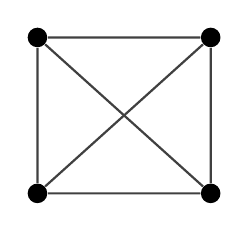
\begin{tikzpicture}[scale=1.1]
        \node[dot] (a) at (0, 1.8) {};
        \node[dot] (b) at (2, 1.8) {};
        \node[dot] (c) at (2, 0) {};
        \node[dot] (d) at (0, 0) {};

        \draw[edge] (a) -- (b) -- (c) -- (d) -- (a);
        \draw[edge] (a) -- (c);
        \draw[edge] (b) -- (d);
    \end{tikzpicture}
    \caption{$K_4$ teljes gráf: 4 csúcs és $\frac{4 \cdot 3}{2} = 6$ él.}
\end{figure}

\begin{feladatdoboz}[9. Feladat: Többlépcsős számolás ($K_6$ teljes gráf)]
Egy sakkbajnokságon 6 versenyző vesz részt, és mindenki mindenkivel pontosan egyszer játszik.
\begin{enumerate}[label=\alph*)]
    \item \textbf{1. lépés:} Hány meccset játszik egyetlen versenyző?
    \item \textbf{2. lépés:} Mennyi a játékosok fokszámainak összege?
    \item \textbf{3. lépés:} Hány mérkőzést játszanak le összesen a bajnokságon?
\end{enumerate}
\end{feladatdoboz}

\begin{megoldasdoboz}[Megoldás a 9. feladathoz]
\begin{enumerate}[label=\alph*)]
    \item Mindenki a másik 5 versenyzővel játszik: $n - 1 = 6 - 1 = \mathbf{5\text{ meccs}}$.
    \item A fokszámok összege: $6 \times 5 = \mathbf{30}$.
    \item A mérkőzések (élek) száma: $|E| = \frac{30}{2} = \frac{6 \cdot 5}{2} = \mathbf{15\text{ mérkőzés}}$.
\end{enumerate}
\end{megoldasdoboz}

\vspace{0.4cm}
% ==============================================================================
% 10. EGYSÉG: FA GRÁFOK
% ==============================================================================
\section{10. Mikro-egység: A fa gráf}

\begin{definiciodoboz}[Fa gráf]
Egy gráfot \textbf{fának} nevezünk, ha \textbf{összefüggő} és \textbf{körmentes}.
\end{definiciodoboz}

\begin{teteldoboz}[Fa éleinek száma]
Minden $n$ csúcsú fa gráf éleinek száma pontosan eggyel kevesebb a csúcsok számánál:
\begin{equation}
    |E| = n - 1
\end{equation}
\end{teteldoboz}

\begin{figure}[H]
    \centering
    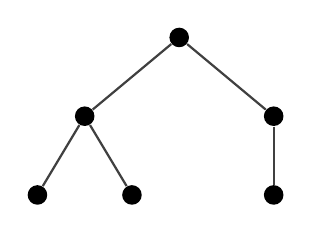
\begin{tikzpicture}[scale=1.0]
        \node[dot] (root) at (2, 2) {};
        \node[dot] (c1) at (0.8, 1) {};
        \node[dot] (c2) at (3.2, 1) {};
        \node[dot] (l1) at (0.2, 0) {};
        \node[dot] (l2) at (1.4, 0) {};
        \node[dot] (l3) at (3.2, 0) {};

        \draw[edge] (root) -- (c1);
        \draw[edge] (root) -- (c2);
        \draw[edge] (c1) -- (l1);
        \draw[edge] (c1) -- (l2);
        \draw[edge] (c2) -- (l3);
    \end{tikzpicture}
    \caption{Egy 6 csúcsú fa: $n = 6$ csúcs, $|E| = 5$ él, körök nélkül.}
\end{figure}

\begin{feladatdoboz}[10. Kérdés: Számérték és Igaz/Hamis]
\textbf{A) Számolás:} Egy számítógépes fa-hálózatban 15 munkaállomás (csúcs) van összekötve. Hány hálózati kábelre (élre) van szükség minimálisan? \\
\textbf{B) Igaz/Hamis:} Ha egy fában behúzunk még egyetlen tetszőleges új élt két csúcs közé, a gráfban garantáltan létrejön egy kör.
\end{feladatdoboz}

\begin{megoldasdoboz}[Megoldás a 10. feladathoz]
\textbf{A) 14 kábelre:} $|E| = n - 1 = 15 - 1 = \mathbf{14}$. \\
\textbf{B) Igaz:} Mivel a fa már eleve összefüggő volt, a két csúcs között korábban is vezetett út; az új él ezt az utat körré zárja.
\end{megoldasdoboz}

\vspace{0.4cm}
% ==============================================================================
% 11. EGYSÉG: KOMPLEMENTER GRÁF
% ==============================================================================
\section{11. Mikro-egység: Komplementer gráf (\texorpdfstring{$\bar{G}$}{G komplementer})}

\begin{definiciodoboz}[Komplementer gráf]
A $G = (V, E)$ gráf \textbf{komplementere} ($\bar{G}$) ugyanazzal a csúcshalmazzal rendelkezik, és két csúcs között akkor és csak akkor van él $\bar{G}$-ben, ha $G$-ben nem volt közöttük él.
\end{definiciodoboz}

Egy gráf és komplementere együtt kiadja a teljes gráfot:
\begin{equation}
    |E(G)| + |E(\bar{G})| = |E(K_n)| = \binom{n}{2}
\end{equation}

\begin{feladatdoboz}[11. Feladat: Számolás]
Egy 5 csúcsú egyszerű $G$ gráfnak 3 éle van. Hány éle van a komplementerének ($\bar{G}$)?
\end{feladatdoboz}

\begin{megoldasdoboz}[Megoldás a 11. feladathoz]
Az 5 csúcsú teljes gráf éleinek száma:
\[
    |E(K_5)| = \frac{5 \cdot 4}{2} = 10.
\]
A komplementer éleinek száma:
\[
    |E(\bar{G})| = 10 - |E(G)| = 10 - 3 = \mathbf{7\text{ él}}.
\]
\end{megoldasdoboz}

\vspace{0.4cm}
% ==============================================================================
% 12. EGYSÉG: EULER-VONAL
% ==============================================================================
\section{12. Mikro-egység: Euler-vonal és Rajzolhatóság}

\begin{definiciodoboz}[Euler-vonal]
Az \textbf{Euler-vonal} olyan élsorozat egy összefüggő gráfban, amely \textbf{minden élt pontosan egyszer} tartalmaz (a ceruza felemelése és vonalismétlés nélkül bejárható).
\begin{itemize}
    \item \textbf{Zárt Euler-vonal:} ugyanabba a csúcsba érkezik vissza, ahonnan indult.
    \item \textbf{Nyílt Euler-vonal:} más csúcsban végződik, mint ahonnan indult.
\end{itemize}
\end{definiciodoboz}

\begin{teteldoboz}[Euler tétele a megrajzolhatóságról]
Összefüggő gráfban:
\begin{enumerate}
    \item \textbf{Zárt Euler-vonal} akkor és csak akkor létezik, ha \textbf{minden csúcs fokszáma PÁROS}.
    \item \textbf{Nyílt Euler-vonal} akkor és csak akkor létezik, ha \textbf{pontosan 2 darab páratlan fokszámú csúcs} van a gráfban. (Ekkor a rajzolást az egyik páratlan csúcsból kell indítani, és a másikban fog befejeződni!)
\end{enumerate}
\end{teteldoboz}

\begin{figure}[H]
    \centering
    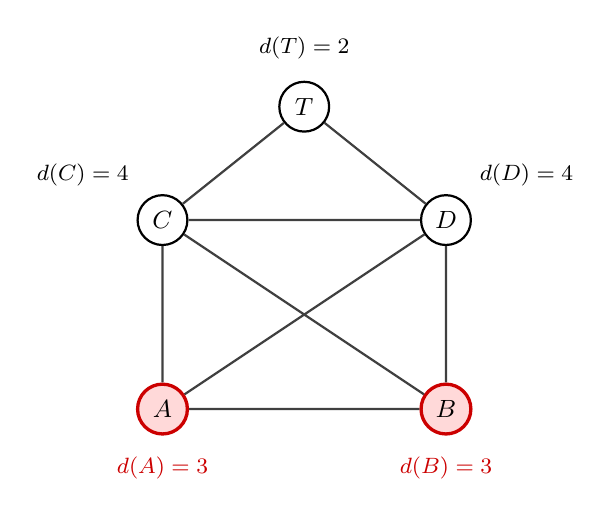
\begin{tikzpicture}[scale=1.2]
        % Itt a szövegben kifejezetten hivatkozunk a csúcsok betűire, ezért betűs címkézést alkalmazunk
        \node[labeledoddvertex] (A) at (0,0) {$A$};
        \node[labeledoddvertex] (B) at (3,0) {$B$};
        \node[labeledvertex] (C) at (0,2) {$C$};
        \node[labeledvertex] (D) at (3,2) {$D$};
        \node[labeledvertex] (T) at (1.5,3.2) {$T$};

        \draw[edge] (A) -- (B) -- (D) -- (C) -- (A) -- (D) -- (T) -- (C) -- (B);

        \node[below=0.15cm of A, text=bvred, font=\footnotesize] {$d(A)=3$};
        \node[below=0.15cm of B, text=bvred, font=\footnotesize] {$d(B)=3$};
        \node[above left=0.1cm of C, font=\footnotesize] {$d(C)=4$};
        \node[above right=0.1cm of D, font=\footnotesize] {$d(D)=4$};
        \node[above=0.15cm of T, font=\footnotesize] {$d(T)=2$};
    \end{tikzpicture}
    \caption{A klasszikus nyitott boríték: az $A$ és $B$ csúcs foka 3 (páratlan), a többi páros. Nyílt Euler-vonal rajzolható $A$-ból $B$-be.}
\end{figure}

\begin{feladatdoboz}[12. Feladat: Többlépcsős döntési feladat (A mélygarázs ellenőrzése)]
Egy éjjeliőrnek végig kell járnia egy telephely összes útszakaszát úgy, hogy minden úton pontosan egyszer halad végig. A telephely kereszteződéseinek fokszámai rendre:
\[
    2,\; 3,\; 2,\; 3,\; 2.
\]
\begin{enumerate}[label=\alph*)]
    \item \textbf{1. kérdés:} Hány darab páratlan fokszámú csomópont található a telephelyen?
    \item \textbf{2. kérdés:} Megvalósítható-e a bejárás egyetlen folyamatos útvonallal?
    \item \textbf{3. kérdés:} Honnan indíthatja az őr az ellenőrzést, és hol fog befejeződni?
\end{enumerate}
\end{feladatdoboz}

\begin{megoldasdoboz}[Megoldás a 12. feladathoz]
\begin{enumerate}[label=\alph*)]
    \item A fokszámok között két darab 3-as van, így \textbf{pontosan 2 páratlan fokszámú csúcs} létezik.
    \item \textbf{Igen}, Euler tétele szerint nyílt Euler-vonal létezik.
    \item A túrát kötelező a két 3-as fofszámú kereszteződés egyikéből indítani, és a másik 3-as fokszámú kereszteződésben fog befejeződni.
\end{enumerate}
\end{megoldasdoboz}

\vspace{0.5cm}
% ==============================================================================
% ÖSSZEFOGLALÓ MIKRO-TÁBLÁZAT
% ==============================================================================
\section{13. Gyors áttekintő kulcstáblázat}

\begin{table}[H]
    \centering
    \resizebox{\linewidth}{!}{%
    \begin{tabular}{lp{6.2cm}c}
        \toprule
        \textbf{Fogalom} & \textbf{Lényeges szabály} & \textbf{Képlet} \\
        \midrule
        \textbf{Kézfogási lemma} & A fokszámok összege mindig páros. & $\sum d(v) = 2|E|$ \\
        \textbf{Páratlan csúcsok} & Számuk minden egyszerű gráfban páros. & -- \\
        \textbf{Teljes gráf ($K_n$)} & Minden csúcs össze van kötve egymással. & $|E| = \frac{n(n-1)}{2}$ \\
        \textbf{Fa gráf} & Összefüggő és körmentes. & $|E| = n - 1$ \\
        \textbf{Komplementer ($\bar{G}$)} & Hiányzó élek a teljes gráfhoz képest. & $|E| + |\bar{E}| = \binom{n}{2}$ \\
        \textbf{Zárt Euler-vonal} & Egyetlen vonallal önmagába visszatérve. & Minden csúcs foka páros \\
        \textbf{Nyílt Euler-vonal} & Egyetlen vonallal más végponttal. & Pontosan 2 páratlan csúcs \\
        \bottomrule
    \end{tabular}%
    }
    \caption{A legfontosabb gráfelméleti mikrotudás egy táblázatban összefoglalva.}
\end{table}

\end{document}
